\title{Self Organizing Systems Exercise 1}
\author{
        Alexander Dobler 01631858\\
        Thomas Kaufmann 01129115 
}
\date{\today}

\documentclass[12pt]{article}

\usepackage{hyperref}
\usepackage{booktabs}
\usepackage{graphics}
\usepackage{multirow}
\usepackage{graphicx}
\usepackage{subcaption}
\usepackage{mwe}

\begin{document}
\maketitle

\section{Introduction \& Problem Description}
For exercise 1 of self-organizing systems we chose the task \textit{Sequence alignment for Genetic Data (DNA Lattice) Anonymization} in which we should solve the DNA lattice anonymization described in \cite{mainpaper} with two metaheuristic techniques from the lecture.
The task is to find a pairing of DNA sequences, such that the sum of distances between two DNA sequences of a pair over all pairs is as small as possible.

More specifically we are given a set of $n$ sequences described by strings which can have different length.
In a first step we have to align these sequences, such that all sequences have the same length.
This is done by introducing a \textit{gap}-characters to increase the length of sequences.
In general this process is called multiple sequence alignment (MSA) and we do not describe how this is done here but rather use a python-library as a black-box tool for this step.
Now, that every sequence has the same length, we can compute the distance between two sequences as described in \cite{mainpaper}.
The last and main step is to combine this set of sequences into pairs, such that the sum of distances of two sequences of pair summed up over all pairs is minimal.
Obviously this is just an application of minimal weighted matching in a complete graph, where a graph is represented by $G=(V,E)$ as follows.
The set $V$ of nodes are described by the sequences and the set $E$ of edges is $V\times V$.
For an edge $e=\{u,v\}$ its weight $w(e)$ is just the distance between the sequences $u$ and $v$.

In the next sections we describe our solution approaches and main results.

\section{Test Data \& Preprocessing}
As base set of data we chose DNA sequences from \url{https://www.kaggle.com/neelvasani/humandnadata} which consists of over 4000 human DNA sequences.
In a next step we created multiple instances of different size by selecting 10-300 random samples of these sequences.
Test-case sizes are always even, such that we do not have to bother about the leftover single sequence.
For each of these instances we performed some preprocessing with the python module \textit{Bio.SeqIO} from the package \textit{Bio} (\url{https://biopython.org/wiki/SeqIO}) and as suggested in ~\cite{mainpaper} computed  multiple sequence alignments with the MSA-toolkit \emph{ClustalW}~\cite{clustalw}. In the last step we compute the cost-matrix between pairs of sequences as described in \cite{mainpaper}.
All of the algorithms described in the next section only use the cost-matrix to compute a pairing.
Although we chose instances of sizes comparable to the work of Bradley~\cite{mainpaper}, as shown below, instances turned out being relatively easily solve where even the relatively simple construction heuristic obtains high quality solutions in little to no execution time. We then further investigated this behavior in more depth and found that a specially structured cost matrix due to the tree-based alignment procedure in \emph{ClustalW} often leads to edge-costs of $0$ between specific pairs in graph, inherently favouring the nature of the DNALA construction heuristic. 

These test-cases can be found in the project under the folder \textit{data}:
Sequence alignments for each test-case are stored in the files \textit{human\_data\_XX.fasta} where \textit{XX} denotes the size of the test-case.
Similarly \textit{human\_data\_XX.cm} stores the cost-matrices in \textit{pickle}-format (\url{https://docs.python.org/3/library/pickle.html}).

\section{DNALA \& Exact Method}
We provide two preliminary methods to solve this problem which are used to benchmark the metaheuristik techniques:
\begin{itemize}
    \item An implementation of the DNALA algorithm as described in \cite{mainpaper} can be found in the \textit{algorithms} directory.
    We did implement the described randomness, but do not use multiple runs of the algorithm, but instead only run the algorithm for a testset once to determine its capability.

    \item As DNALA is only a heuristic and is not guaranteed to find an optimal solution we furthermore use a maximum weighted matching provided by the package \textit{networkx} (\url{https://networkx.org/documentation/stable//index.html}) to compute an exact solution used for optimality gaps in benchmarking.
\end{itemize}

\section{Genetic Algorithm}
The first metaheuristic technique with which we solve the problem is a genetic algorithm.
For this we use the \textit{deap}-package for python (\url{https://deap.readthedocs.io/en/master/}) which provides a framework for creating genetic algorithms.
The well-know genetic algorithm compononents are implemented as follows:
\begin{itemize}
    \item \textbf{Solution representation}: A solution consists of $\frac{n}{2}$ pairs such that each node (sequence) appears in exactly one pair.
    \item \textbf{Fitness}: The fitness is just the sum of distances between pairs of points. 
    This in fact also represents the value of a weighted matching the corresponding weighted matching.
    \item \textbf{Crossover}: 
    \item \textbf{Mutation}: Selects a random pair of matchings based on the mutation probability and the best two-opt move in the induced subgraph. 
\end{itemize}
Furthermore we have the option to select different population sizes and mutation rates for running the algorithm.

\section{Ant Colony Optimization}
At first we did not know how to solve the problem with ant colony optimization.
But then we realized that a weighted matching in a complete graph is just a tour visiting every vertice where every second edge will have weight 0.
This was really convenient, as ant colony optimization is well-known to perform well on the TSP-problem.
Furthermore there are a lot of implementations available, which provide ACO-methods to solve the TSP-problem.
For our purposes it was enough to alter the implementation provided by the \textit{pants}-package (\url{https://pypi.org/project/ACO-Pants/}) in a way, such that we could solve the minimum weighted matching problem.

Our alteration can be described as follows.
When solving the TSP-problem every ant starts at a specific node and tries to find a best tour.
This means that at a specific point of the algorithm each ant has currently visited an acyclic path.
Now this path has either even or odd length.
This means when an ant can chose its next edge there are two different strategies:
\begin{itemize}
    \item If the path until now has even length, then chose the usual strategy to select the next node to visit (pheromones in ACO with $\alpha$- and $\beta$-values).
    \item If the path until now has odd length, then go to any not yet visited node.
    This resembles the fact that every other edge of the tour will have weight 0.
\end{itemize}
Of course we also have to alter the cost of a tour, in partical that every other edge has weight 0, to guide the algorithm to an optimal solution.

One might think that this construction of an algorithm to solve the minimum weighted matching problem is pretty superficial, but we will see that its performance is not too bad.

\section{Local Search}
two-opt neighborhood
first fit step function 
...



\section{Results \& Conclusion}

info:
300s execution time
optimality gap as scale invariant measure for distance to the optimum

median execution time until termination
median iteration until optimum was obtained 

iterations are 0 indexed, so sometimes, just fyi

\begin{table}
\centering
\resizebox{\columnwidth}{!}{%
\begin{tabular}{llr|rrrr|rrrr}
\toprule
   &     &          & \multicolumn{4}{|c|}{Without Local Search} & \multicolumn{4}{|c}{With Local Search} \\
   &     &  Optimum &  Fitness &    Gap &   Time &  $I_{opt}$ &  Fitness &   Gap &   Time &  $I_{opt}$ \\
ALG & n &          &          &        &        &            &          &       &        &            \\
\midrule
GA & 10  &     1994 &     1994 &   0.00 &   0.00 &          0 &     1994 &  0.00 &   0.00 &          0 \\
   & 20  &    11758 &    11758 &   0.00 &   1.00 &         14 &    11758 &  0.00 &   0.00 &          0 \\
   & 30  &    19032 &    19032 &   0.00 &   3.00 &         31 &    19032 &  0.00 &   1.00 &          0 \\
   & 40  &    20892 &    20892 &   0.00 &   6.00 &         59 &    20892 &  0.00 &   3.00 &          0 \\
   & 50  &    34198 &    34198 &   0.00 &  20.00 &        148 &    34198 &  0.00 &   5.00 &          0 \\
   & 60  &    42382 &    42382 &   0.00 &  29.00 &        161 &    42382 &  0.00 &  12.00 &          1 \\
   & 70  &    47234 &    47244 &   0.02 & 300.00 &        170 &    47234 &  0.00 &  18.00 &          1 \\
   & 80  &    53538 &    54812 &   2.38 & 300.00 &        207 &    53538 &  0.00 &  19.00 &          2 \\
   & 90  &    69731 &    69909 &   0.26 & 300.00 &        337 &    69731 &  0.00 &  25.00 &          2 \\
   & 100 &    83495 &    92065 &  10.26 & 300.00 &        217 &    83495 &  0.00 &  62.00 &          4 \\
   & 150 &   104772 &   178368 &  70.24 & 300.00 &        136 &   104772 &  0.00 & 225.00 &          7 \\
   & 200 &   130178 &   315378 & 142.27 & 300.00 &        131 &   130820 &  0.49 & 300.00 &          8 \\
   \midrule
ACO & 10  &     1994 &     1994 &   0.00 &   0.00 &          0 &     1994 &  0.00 &   0.00 &          0 \\
   & 20  &    11758 &    11758 &   0.00 &   0.00 &          0 &    11758 &  0.00 &   0.00 &          0 \\
   & 30  &    19032 &    19032 &   0.00 &   0.00 &          2 &    19032 &  0.00 &   0.00 &          0 \\
   & 40  &    20892 &    20892 &   0.00 &  10.00 &         88 &    20892 &  0.00 &   0.00 &          0 \\
   & 50  &    34198 &    34320 &   0.36 & 300.00 &        280 &    34198 &  0.00 &   1.00 &          0 \\
   & 60  &    42382 &    44310 &   4.55 & 300.00 &        317 &    42382 &  0.00 &   2.00 &          0 \\
   & 70  &    47234 &    51766 &   9.59 & 300.00 &        623 &    47234 &  0.00 &   3.00 &          0 \\
   & 80  &    53538 &    60872 &  13.70 & 300.00 &        587 &    53538 &  0.00 &   4.00 &          0 \\
   & 90  &    69731 &    82387 &  18.15 & 300.00 &        150 &    69731 &  0.00 &   6.00 &          0 \\
   & 100 &    83495 &   107141 &  28.32 & 300.00 &        257 &    83495 &  0.00 &  42.00 &          5 \\
   & 150 &   104772 &   150908 &  44.03 & 300.00 &         68 &   107586 &  2.69 & 300.00 &         24 \\
   & 200 &   130178 &   217644 &  67.19 & 300.00 &         36 &   170190 & 30.74 & 300.00 &         17 \\
   \midrule
DNALA & 10  &     1994 &     1994 &   0.00 &   0.00 &          0 &     1994 &  0.00 &   0.00 &          1 \\
   & 20  &    11758 &    11758 &   0.00 &   0.00 &          0 &    11758 &  0.00 &   0.00 &          1 \\
   & 30  &    19032 &    19032 &   0.00 &   0.00 &          0 &    19032 &  0.00 &   0.00 &          1 \\
   & 40  &    20892 &    22066 &   5.62 &   0.00 &          0 &    21164 &  1.30 &   0.00 &          1 \\
   & 50  &    34198 &    35336 &   3.33 &   0.00 &          0 &    34198 &  0.00 &   0.00 &          1 \\
   & 60  &    42382 &    44666 &   5.39 &   0.00 &          0 &    42890 &  1.20 &   0.00 &          1 \\
   & 70  &    47234 &    47252 &   0.04 &   0.00 &          0 &    47244 &  0.02 &   0.00 &          1 \\
   & 80  &    53538 &    55448 &   3.57 &   0.00 &          0 &    53538 &  0.00 &   0.00 &          1 \\
   & 90  &    69731 &    71779 &   2.94 &   0.00 &          0 &    69747 &  0.02 &   0.00 &          1 \\
   & 100 &    83495 &    86513 &   3.61 &   0.00 &          0 &    85293 &  2.15 &   0.00 &          1 \\
   & 150 &   104772 &   105824 &   1.00 &   0.00 &          0 &   104940 &  0.16 &   0.00 &          1 \\
   & 200 &   130178 &   134640 &   3.43 &   0.00 &          0 &   130194 &  0.01 &   0.00 &          1 \\

\bottomrule
\end{tabular}%
}
\end{table}


  \begin{figure*}
        \centering
        \begin{subfigure}[b]{0.475\textwidth}
            \centering
            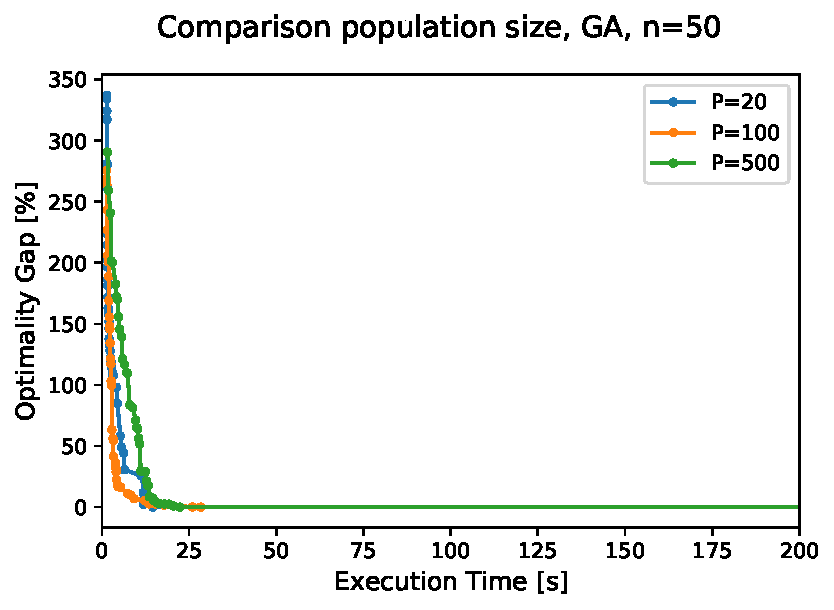
\includegraphics[width=\textwidth]{figures/ga_50_population_comparison.pdf}
            \caption%
            {{\small }}    
            \label{fig:mean and std of net14}
        \end{subfigure}
        \hfill
        \begin{subfigure}[b]{0.475\textwidth}  
            \centering 
            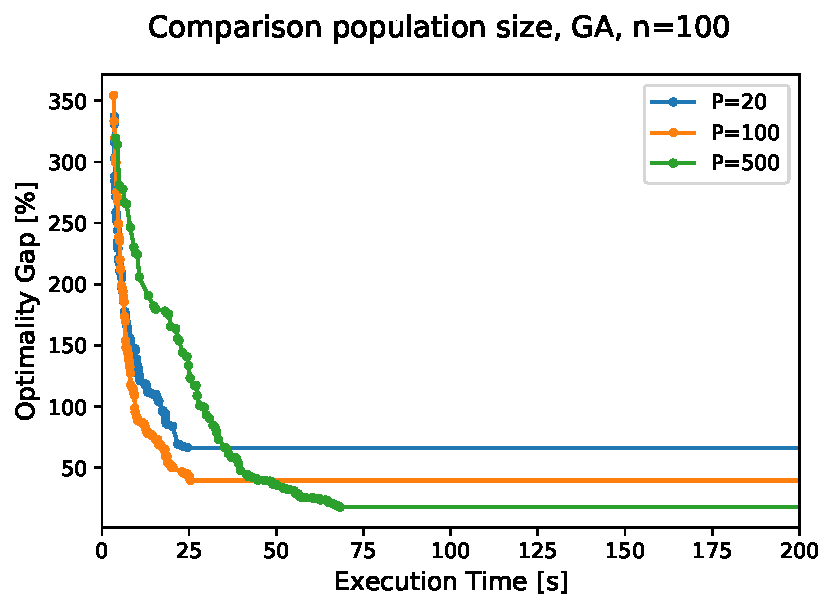
\includegraphics[width=\textwidth]{figures/ga_100_population_comparison.pdf}
            \caption%
            {{\small }}     
            \label{fig:mean and std of net24}
        \end{subfigure}
        \vskip\baselineskip
        \begin{subfigure}[b]{0.475\textwidth}   
            \centering 
            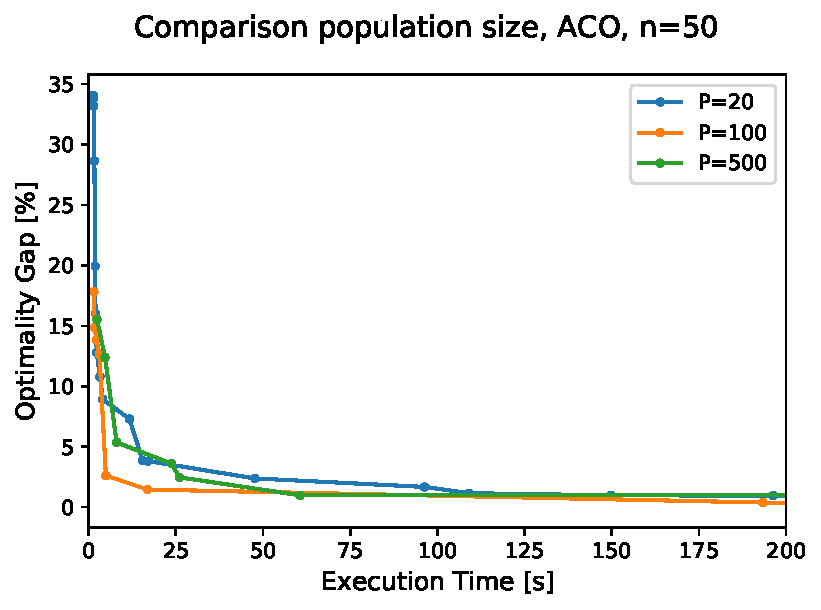
\includegraphics[width=\textwidth]{figures/aco_50_population_comparison.pdf}
            \caption%
            {{\small }}      
            \label{fig:mean and std of net34}
        \end{subfigure}
        \hfill
        \begin{subfigure}[b]{0.475\textwidth}   
            \centering 
            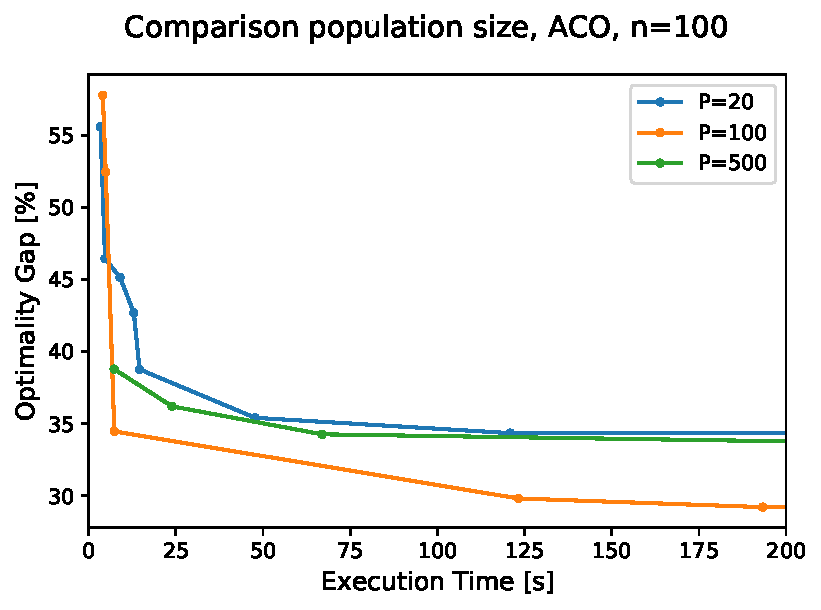
\includegraphics[width=\textwidth]{figures/aco_100_population_comparison.pdf}
            \caption%
            {{\small }}    
            \label{fig:mean and std of net44}
        \end{subfigure}
        \caption
        {\small Optimality gap over time for different population sizes on instances with $n=50$ and $n=100$ vertices. } 
        \label{fig:mean and std of nets}
    \end{figure*}




 \begin{figure*}
        \centering
        \begin{subfigure}[b]{0.475\textwidth}
            \centering
            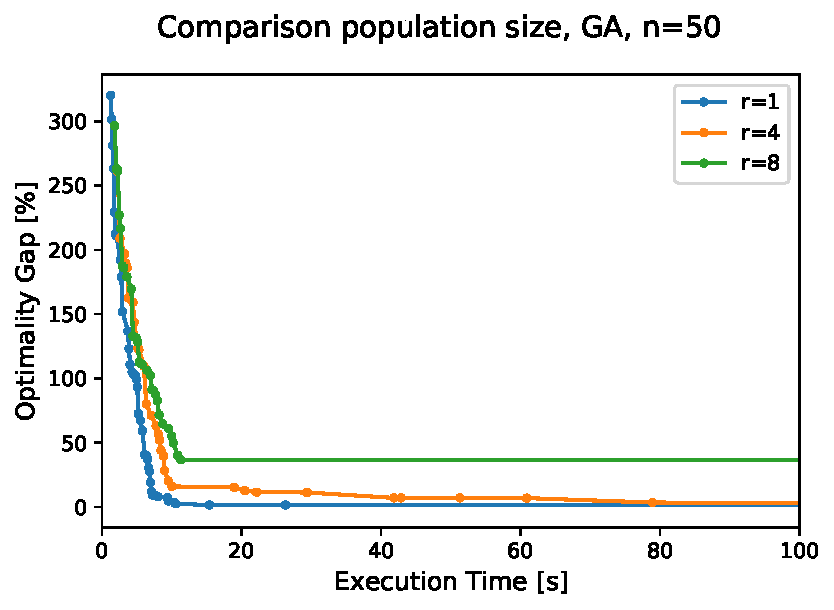
\includegraphics[width=\textwidth]{figures/ga_50_mutation_rate_comparison.pdf}
            \caption%
            {{\small }}    
            \label{fig:mean and std of net14}
        \end{subfigure}
        \hfill
        \begin{subfigure}[b]{0.475\textwidth}  
            \centering 
            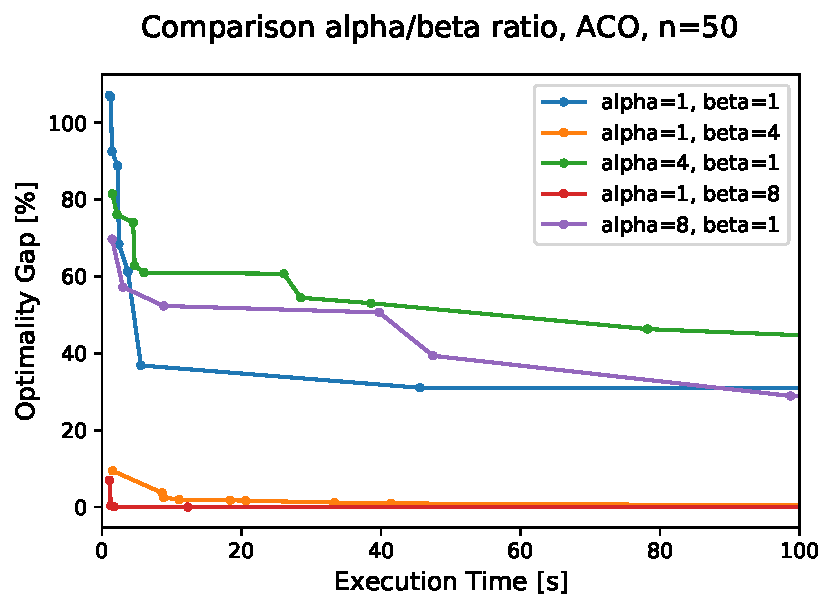
\includegraphics[width=\textwidth]{figures/aco_50_alpha_beta_ratio_comparison.pdf}
            \caption%
            {{\small }}     
            \label{fig:mean and std of net24}
        \end{subfigure}
        \caption
        {\small Optimality gap over time for different population sizes on instances with $n=50$ and $n=100$ vertices. } 
        \label{fig:mean and std of nets}
    \end{figure*}


todo add some experiments with different parameters for population size


\bibliographystyle{abbrv}
\bibliography{main}

\end{document}
  